
\documentclass[10pt,twocolumn]{article}

% Följande rad ska göra det möjligt att använda svenska bokstäver, som å, ä, ö. Kravet är 
% då att filen sparas i UTF-8-format. Om detta inte fungerar för dig, så kan du alltid 
% använda dig av {\aa} för å, \"a för ä och \"o för ö.
\usepackage[utf8]{inputenc}

% Följande väljer typsnitt som är kloner av Times New Roman, Helvetica och lämpliga till
% dem anpassade matematiktypsnitt.
\usepackage{newtxtext}
\usepackage{newtxmath}

%  Följande tillhandahåller miljön spver­ba­tim som är lämplig för att typsätta programkod.
\usepackage{spverbatim}

% To include images
\usepackage{graphicx}

% For syntax highlighted code
\usepackage{listings}
\usepackage{xcolor}
\usepackage{color}
\usepackage{icomma}
\definecolor{dkgreen}{rgb}{0,0.6,0}
\definecolor{gray}{rgb}{0.5,0.5,0.5}
\definecolor{mauve}{rgb}{0.58,0,0.82}
\lstset{%
    aboveskip=3mm,
    belowskip=3mm,
    showstringspaces=false,
    columns=flexible,
    basicstyle={\small\ttfamily},
    numbers=none,
    numberstyle=\tiny\color{red},
    keywordstyle=\color{blue},
    commentstyle=\color{dkgreen},
    stringstyle=\color{mauve},
    breaklines=true,
    breakatwhitespace=true,
    tabsize=3
}

% Convenience commands
\newcommand{\echodelay}{\tau}
\newcommand{\lpfilter}{\mathcal{H}_{LP}^{5 \text{kHz}}}

\DeclareMathSymbol{.}{\mathord}{letters}{"3B}
\usepackage{siunitx}

% \DeclareMathSymbol{,}{\mathord}{letters}{"3B}

\raggedbottom
\sloppy

\title{Laborationsrapport i TSKS10 \emph{Signaler, Information och Kommunikation}}

\author{Frans Skarman \\ frask812, 9509085552 }

\date{6 Juni, 2017}

\begin{document}

\maketitle

\section{Inledning}

Denna laboration gick ut på att demodulera en iq-modulerad signal som var given
tillsammans med andra signaler i en .wav fil. I och Q delen av signalen skulle
bestå av två separata melodier följt av två ordspråk.

Utöver den sökta signalen innehöll även datan två signaler med andra bärfrekvenser
och ett simulerat eko med okänd tidsfördröjning. Hela signalen var fördröjd
för att simulera signalens restid och osynkroniserade klockor mellan sändare och mottagare.
Datan innehöll
även två stycken cosinus-signaler med närliggande frekvenser som kunde utnyttjas för
att bestämma ekots fördröjning. Frekvenserna $f_1$ och $f_2$ för dessa signaler 
skulle också bestämmas.

I uppgiften ingick en lista på vilka bärfrekvenser huvudsignalerna kunde använda.
Det var även givet att amplituden på den ekande signalen var $0.9 x(t-\echodelay)$
där $x(t)$ den skickade signalen och $\echodelay$ är ekots tidsfördröjning som var
mindre än $500 \text{ ms}$.

Den givna datans samplingstakt $f_s$ var $400 \text{ kHz}$



\section{Metod}

% Inläsning av signaler

Alla beräkingar gjordes med python-biblioteken scipy och numpy. För att lyssna på de demodulerade
signalerna användes initialt programmet audacity men det byttes senare ut mot python-biblioteket
sounddevice.

\subsection{Bestämning av bärfrekvens}

Det första som gjordes var att fouriertransformera den givna signalen, $x_{given}(t)$, och plotta
dess spektrum. Genom att analysera spektrumet visades det att signalen bestog av tre
delsignaler med frekvenser $75 \text{ kHz}$, $115 \text{ kHz}$ och $151 \text{ kHz}$ samt två cosinussignaler med 
frekvenser $160500 \text{ Hz}$ och $160501 \text{ Hz}$. Signalens spektrum kan ses i Figur \ref{fig:spectrum}.

\begin{figure}[h]
    \centering
    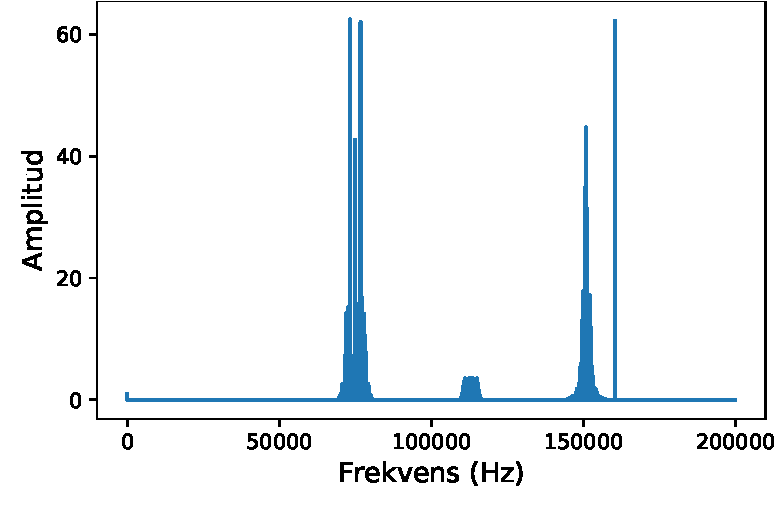
\includegraphics[width=0.85\linewidth]{spectrum.pdf}
    \caption{Amplitudspektrum för $x_{given}(t)$}
    \label{fig:spectrum}
\end{figure}

För att hitta vilken av de tre huvudsignalerna som innehöll den sökta informationen
skrevs de första stegen av IQ-demodulationen. Denna
funktion multiplicerade den givna signalen $x_{given}(t)$ med signalen $\cos(2\pi f_c t)$ där $f_c$
är bärfrekvensen för signalen. Den resulterande signalen filtrerades sedan med ett 
butterworth-lågpassfilter med gränsfrekvens $5 \text{ kHz}$. Gränsfrekvensen valdes eftersom
att signalernas bandbredd var ungefär $5 \text{ kHz}$.

Den demodulerade signalen $x(t)$ beräknades altså enligt

\begin{equation}
    x(t) = \lpfilter\{ x_{given}(t) \cdot \cos(2\pi f_c t) \}
\end{equation}




Denna funktion användes för att demodulera de tre nyttosignalerna och resultatet spelades
upp med audacity. En av signalerna visade sig vara brus, en var fågelkvitter och en började
med vad som lät som två överlagrade melodier. Den sistnämnda signalen hade bärfrekvensen 151kHz
och är signalen som resten av rapporten kommer att analysera.




\subsection{Ekotidsfördröjning}
Nästa steg som gjordes var att hitta tidsfördröjningen
mellan den mottagna signalen och dess eko, $\echodelay=\tau_2-\tau_2$.
För att göra detta autokorrelerades de $100000$ första samplen
av signalen med de efterföljande $400000$ vilket med datans samplingstakt motsvarar en sekund.

Autokorrelationen gav ett maximalt värde vid sampel $63999$ vilket med den initiala förskjutningen på
$100000$ sampel gav ekots tidsfördröjning $\echodelay=163999$ sampel eller $0.41 \text{ s}$.

\subsection{Fullständing IQ demodulering}

För att fullständigt demodulera de två I och Q komponenterna, $x_i(t)$ och $x_q(t)$, beräknades signalerna 
$\hat{x}_Q$ och $\hat{x}_I$ enlgit följande formler där $f_c = 151\text{ kHz}$:

\[
    \hat{x}_I(t) = \lpfilter\{ 2 \bar{x}(t) \cos(2\pi f_c t) \}
\]
\[
    \hat{x}_Q(t) = \lpfilter\{ 2 \bar{x}(t) \sin(2\pi f_c t) \}
\]

Eftersom att mottagarens klocka inte var synkroniserad med sändaren blandades I och Q komponenterna
i den mottagna signalen enligt ekvation \ref{eq:iq_mix} där $\delta$ är tidsfördröjningen mellan sändaren och mottagaren.

\begin{equation}
    \label{eq:iq_mix}
    \left[
        \begin{array}{c}
            \hat{x}_I(t) \\
            \hat{x}_Q(t)
        \end{array}
    \right]
    =
    \left[
        \begin{array}{cc}
            \cos(\delta) & \sin(\delta) \\
            -\sin(\delta) & \cos(\delta)
        \end{array}
    \right]
    \left[
        \begin{array}{c}
            x_I(t) \\
            x_Q(t)
        \end{array}
    \right]
\end{equation}

För att beräkna de skickade signalerna $x_I(t)$ och $x_Q(t)$ användes ekvation \ref{eq:iq_demix} som
fanns med i facit till uppgift 2.13 i kursboken.
\begin{equation}
    \label{eq:iq_demix}
    \left[
        \begin{array}{c}
            x_I(t) \\
            x_Q(t)
        \end{array}
    \right]
    =
    \left[
        \begin{array}{cc}
            \cos(\delta) & -\sin(\delta) \\
            \sin(\delta) & \cos(\delta)
        \end{array}
    \right]
    \left[
        \begin{array}{c}
            \hat{x}_I(t) \\
            \hat{x}_Q(t)
        \end{array}
    \right]
\end{equation}


Eftersom att ekvation \ref{eq:iq_mix} motsvarar en vridning så räckte det med att hitta ett 
$0 \leq \delta \leq 2\pi$ som separerade I- och Q-komponenterna.
Eftersom att det i den här labben inte var viktigt att hitta vilken av de två mottagna signalerna som
motsvarar de skickade I- och Q-signalerna utan bara att separera signalerna, och att det för ljud inte spelar
någon roll om fasen är förskjuten ett halvt varv räckte det med att hitta ett 
$0 \leq \delta \leq \frac{\pi}{2}$

Detta gjordes genom att stega igenom olika värden på $\delta$ och hitta ett värde
där de två signalerna var så separerade att man kunde höra de två ordspråken. Detta gav 
$\delta=\frac{3\pi}{8}$.

\subsection{Ekoborttagning}

Det sista som gjordes var att ta bort ekot från de två demodulerade signalerna.

Eftersom att ekot inte påverkar de första $\echodelay$ sampeln kunde de slutgiltiga signalerna
$\bar{x}_I(t)$ och $\bar{x}_Q(t)$ beräknas enligt
\[
    \bar{x}_I(t) =
    \begin{cases}
        {x_I(t)                        & \quad \text{Om } t < \echodelay \\
        {x_I(t) - 0.9 \bar{x}_I(t-\echodelay)  & \quad \text{Annars} \\
    \end{cases}
\]
\[
    \bar{x}_Q(t) =
    \begin{cases}
        {x_Q(t)                        & \quad \text{Om } t < \echodelay \\
        {x_Q(t) - 0.9 \bar{x}_Q(t-\echodelay)  & \quad \text{Annars} \\
    \end{cases}
\]



\section{Resultat}

Den sökta informationen är:
\begin{itemize}
    \item Bärfrekvensen för nyttosignalen är $f_c=151 \text{ kHz}$
    \item Differensen $\tau_2-\tau_1=410 \text{ ms}$
    \item Frekvenserna för de två cosinussignalerna är $f_1=160500 \text{ Hz}$ och $f_2=160500 \text{ Hz}$
    \item Första ordspråket är "Vart man än vänder sig, så har man ändan bak"
    \item Andra ordspråket är "Tala är silver, tiga är guld"
\end{itemize}

\clearpage

\onecolumn
\section*{Min Python-kod:}
\lstinputlisting[language=Python]{../main.py}

\end{document}
